\hypertarget{project-plan}{%
\section{Project Plan}\label{project-plan}}

Thien Nguyen

Supervisor: Stefan Dantchev

Department of Computer Science, Durham University

\hypertarget{description}{%
\subsection{Description}\label{description}}

Draughts AI players are currently designed to play at a fixed ability.
While it has produced very competitive and intelligent players, they
require tweaks in order to improve its performance. By combining Neural
Networks and Genetic Algorithms, this issue could possibly be solved by
creating a player that can grow in ability over time.

\hypertarget{preliminary-preparation}{%
\subsection{Preliminary Preparation}\label{preliminary-preparation}}

\begin{itemize}
\tightlist
\item
  A primer on the game of Draughts and game strategies for board
  evaluations
\item
  A cohesive understanding of Convolutional Neural Networks
\item
  A comprehensive understanding of Genetic Algorithms
\item
  A comprehensive understanding of relevant programming languages and/or
  frameworks that will be needed for implementation.
\end{itemize}

\hypertarget{research-question}{%
\subsection{Research Question}\label{research-question}}

Can we produce a similarly performant draughts by using seperate
classifiers for the different stages of the game?

\hypertarget{deliverables}{%
\subsection{Deliverables}\label{deliverables}}

\hypertarget{minimum}{%
\subsubsection{Minimum}\label{minimum}}

\begin{itemize}
\tightlist
\item
  Implement a CNN
\item
  Implement a Checkers Game Interface
\item
  Implement a genetic algorithm with an evaluation function that
  consists of a round robin tournament against the population of CNN
  Evaluators.
\item
  Implement a mini-max algorithm that chooses moves.
\end{itemize}

\hypertarget{intermediate}{%
\subsubsection{Intermediate}\label{intermediate}}

\begin{itemize}
\tightlist
\item
  A user-friendly interface to play against the AI
\item
  A monte-carlo search of the move space.
\item
  Analysis of Crossover methods (within Genetic Algorithms)
\item
  Analysis of Mutaiton methods (within Genetic Algorithms)
\end{itemize}

\hypertarget{advanced}{%
\subsubsection{Advanced}\label{advanced}}

\begin{itemize}
\tightlist
\item
  Convolutional Neural Network Layer analysis
\item
  The resulting AI can play to an ELO of at least 1200.
\end{itemize}

\hypertarget{project-plan-1}{%
\subsection{Project Plan}\label{project-plan-1}}

For each of the objectives, it would not be difficult to adjust the
dates due to the flexibility of the project; the majority of the basic
objectives can be implemented without dependency on others. It may be
the case that the minimum subobjectives can be implemented in parallel.

Due to the nature of the project, various tweaks will need to be applied
to the different components of the system to optimise performance.
However, this is left for the intermediate and advanced objectives,
where it is assumed that it would be made possible during the system
implementation during the basic objectives.

\begin{figure}
\centering
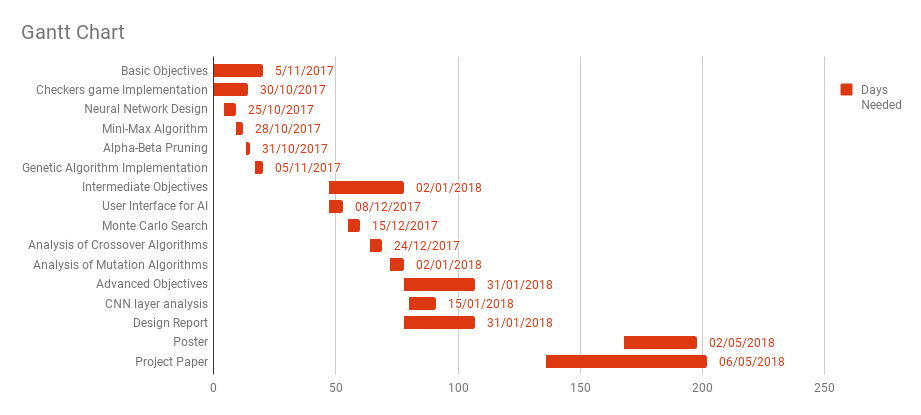
\includegraphics{chart.png}
\caption{Chart}
\end{figure}
